% A LaTeX template for ARTICLE version of the MSc Thesis submissions to 
% Politecnico di Milano (PoliMi) - School of Industrial and Information Engineering
%
% S. Bonetti, A. Gruttadauria, G. Mescolini, A. Zingaro
% e-mail: template-tesi-ingind@polimi.it
%
% Last Revision: October 2021
%
% Copyright 2021 Politecnico di Milano, Italy. Inc. NC-BY

\documentclass[12pt,a4paper]{article} 

%------------------------------------------------------------------------------
%	REQUIRED PACKAGES AND  CONFIGURATIONS
%------------------------------------------------------------------------------
% PACKAGES FOR TITLES
\usepackage{titlesec}
\usepackage{color}

% PACKAGES FOR LANGUAGE AND FONT
\usepackage[utf8]{inputenc}
\usepackage[english]{babel}
\usepackage[T1]{fontenc} % Font encoding

% PACKAGES FOR IMAGES
\usepackage{graphicx}
\graphicspath{{Images/}}
\usepackage{eso-pic} % For the background picture on the title page
\usepackage{subfig} % Numbered and caption subfigures using \subfloat
\usepackage{caption} % Coloured captions
\usepackage{transparent}

% STANDARD MATH PACKAGES
\usepackage{amsmath}
\usepackage{amsthm}
\usepackage{bm}
\usepackage[overload]{empheq}  % For braced-style systems of equations

% PACKAGES FOR TABLES
\usepackage{tabularx}
\usepackage{longtable} % tables that can span several pages
\usepackage{colortbl}

% PACKAGES FOR ALGORITHMS (PSEUDO-CODE)
\usepackage{algorithm}
\usepackage{algorithmic}

% PACKAGES FOR REFERENCES & BIBLIOGRAPHY
\usepackage[colorlinks=true,linkcolor=black,anchorcolor=black,citecolor=black,filecolor=black,menucolor=black,runcolor=black,urlcolor=black]{hyperref} % Adds clickable links at references
\usepackage{cleveref}
\usepackage[authoryear,round]{natbib} % Square brackets, citing references with numbers, citations sorted by appearance in the text and compressed
%\bibliographystyle{plain} % You may use a different style adapted to your field
\bibliographystyle{elsarticle-harv}
% PACKAGES FOR THE APPENDIX
\usepackage{appendix}

% PACKAGES FOR ITEMIZE & ENUMERATES 
\usepackage{enumitem}

% OTHER PACKAGES
\usepackage{amsthm,thmtools,xcolor} % Coloured "Theorem"
\usepackage{comment} % Comment part of code
\usepackage{fancyhdr} % Fancy headers and footers
\usepackage{lipsum} % Insert dummy text
\usepackage{tcolorbox} % Create coloured boxes (e.g. the one for the key-words)
\usepackage{amssymb}
\usepackage{textcomp}
\usepackage{booktabs}


%-------------------------------------------------------------------------
%	NEW COMMANDS DEFINED
%-------------------------------------------------------------------------
% EXAMPLES OF NEW COMMANDS -> here you see how to define new commands
\newcommand{\bea}{\begin{eqnarray}} % Shortcut for equation arrays
\newcommand{\eea}{\end{eqnarray}}
\newcommand{\e}[1]{\times 10^{#1}}  % Powers of 10 notation
\newcommand{\mathbbm}[1]{\text{\usefont{U}{bbm}{m}{n}#1}} % From mathbbm.sty
\newcommand{\pdev}[2]{\frac{\partial#1}{\partial#2}}
% NB: you can also override some existing commands with the keyword \renewcommand

%----------------------------------------------------------------------------
%	ADD YOUR PACKAGES (be careful of package interaction)
%----------------------------------------------------------------------------


%----------------------------------------------------------------------------
%	ADD YOUR DEFINITIONS AND COMMANDS (be careful of existing commands)
%----------------------------------------------------------------------------


% Do not change Configuration_files/config.tex file unless you really know what you are doing. 
% This file ends the configuration procedures (e.g. customizing commands, definition of new commands)
\input{Configuration_files/config}

% Insert here the info that will be displayed into your Title page 
% -> title of your work
\renewcommand{\title}{Title}
% -> author name and surname
\renewcommand{\author}{Name Surname}
% -> MSc course
% \newcommand{\course}{Xxxxxxxxxxxx Engineering - Ingegneria Xxxxxxxxxxxx}
% -> advisor name and surname
\newcommand{\advisor}{Prof. Name Surname}
% IF AND ONLY IF you need to modify the co-supervisors you also have to modify the file Configuration_files/title_page.tex (ONLY where it is marked)
\newcommand{\firstcoadvisor}{Name Surname} % insert if any otherwise comment
\newcommand{\secondcoadvisor}{Name Surname} % insert if any otherwise comment
% -> author ID
\newcommand{\ID}{Student ID}
% -> academic year
\newcommand{\YEAR}{20XX-20XX}
% -> abstract (only in English)
\renewcommand{\abstract}{Bayesian spatial clustering methods partition geographic areas into latent groups while accounting for spatial dependence. In this work, we focus on spatial areal data observed for a single year (2022) and study provincial differences in women’s labour market participation across Italy. We model spatial dependence through the conditional autoregressive (CAR) prior of \cite{Leroux_2000}. We then perform model based clustering by fitting a Bayesian finite mixture model, where latent component memberships define province level clusters, and we examine whether provinces share similar effects of ECEC services on women's employment profile.}

% -> key-words (only in English)
\newcommand{\keywords}{here, the keywords, of your thesis}

%-------------------------------------------------------------------------
%	BEGIN OF YOUR DOCUMENT
%-------------------------------------------------------------------------
\begin{document}

%-----------------------------------------------------------------------------
% TITLE PAGE
%-----------------------------------------------------------------------------
% Do not change Configuration_files/TitlePage.tex (Modify it IF AND ONLY IF you need to add or delete the Co-advisors)
% This file creates the Title Page of the document
% DO NOT REMOVE SPACES BETWEEN LINES!

\AddToShipoutPicture*{\BackgroundPic}

\hspace{-0.6cm}
\includegraphics[width=0.6\textwidth]{logo_polimi_ing_indinf.eps}

\vspace{-1mm}
\Large{\textbf{\color{bluePoli}{Spatial Clustering of Spatial Data}}}\\

\vspace{-0.2cm}
\fontsize{0.3cm}{0.5cm}\selectfont \bfseries \textsc{\color{bluePoli} an application to early childhood education and care and their impact on women’s labour market}\\

\vspace{-0.2cm}
\large{\textbf{Tommaso Alessio Baresi, Luca Perego, Paul Poupeau, Leonardo Tisato, Anh Chi Tuan, Alexis Toppé}}

\small \normalfont

\vspace{11pt}

\centerline{\rule{1.0\textwidth}{0.4pt}}

\begin{center}
\begin{minipage}[t]{.24\textwidth}
\begin{minipage}{.90\textwidth}
\noindent
\scriptsize{\textbf{Advisors:}} \\
Giulio Beltramin \\
Simone Colombara \\
\\
% \textbf{Co-advisors:} \\ % leave it if any co-advisor otherwise comment
% \firstcoadvisor \\ % leave it if any co-advisor otherwise comment
% \secondcoadvisor \\ % leave it if you have more that one co-advisor otherwise comment (if you have more than two co-advisors just copy&paste this line writing \thirdcoadvisor, \fourthcoadvisor, ecc. (REMEMBER to modify also the main.txt)
\\ % leave it if any co-advisor otherwise comment
\textbf{Academic year:} \\
2025-2026 \\
\\
\end{minipage}
\end{minipage}% This must go next to `\end{minipage}`
\begin{minipage}{.74\textwidth}
\noindent \textbf{\color{bluePoli} Abstract:} {\abstract}
\end{minipage}
\end{center}

\vspace{15pt}

\begin{tcolorbox}[arc=0pt, boxrule=0pt, colback=bluePoli!60, width=\textwidth, colupper=white]
    \textbf{Key-words: Bayesian Spatial Clustering, CAR Prior, Sparse Mixture Model}
\end{tcolorbox}

\vspace{12pt}


\input{chapters/introduction}
\section{Exploratory Data Analysis}
\label{sec:explorator_data_analysis}
Data are collected from official statistical sources, primarily the Italian National Institute of Statistics (ISTAT), including the ISTAT Data Warehouse, the Permanent Census of Population and Housing, and \textit{Demografia in cifre}. Additional information was obtained from Eurostat and \textit{Il Sole 24 Ore, Qualità della vita} dataset.\\

This study focuses on 107 Italian provinces. For each of them, the data includes a total of 47 variables, representing different socio-economic measurements\footnote{The complete list of variables and their description is presented in Appendix A.}. \\
Since we want to analyze how ECEC services influence the women's labor market, our response variable is the women's employment rate.
Figure~\ref{fig:heatmap1} shows the spatial distribution of \texttt{fem\_empl\_rate}, defined as the ratio between the number of working women of working age (15-64 years old) and the total number of women of working age, and \texttt{coverage}, defined as the number of available children services over the number of children (0-2 years old):

\begin{figure}[h]
    \centering
    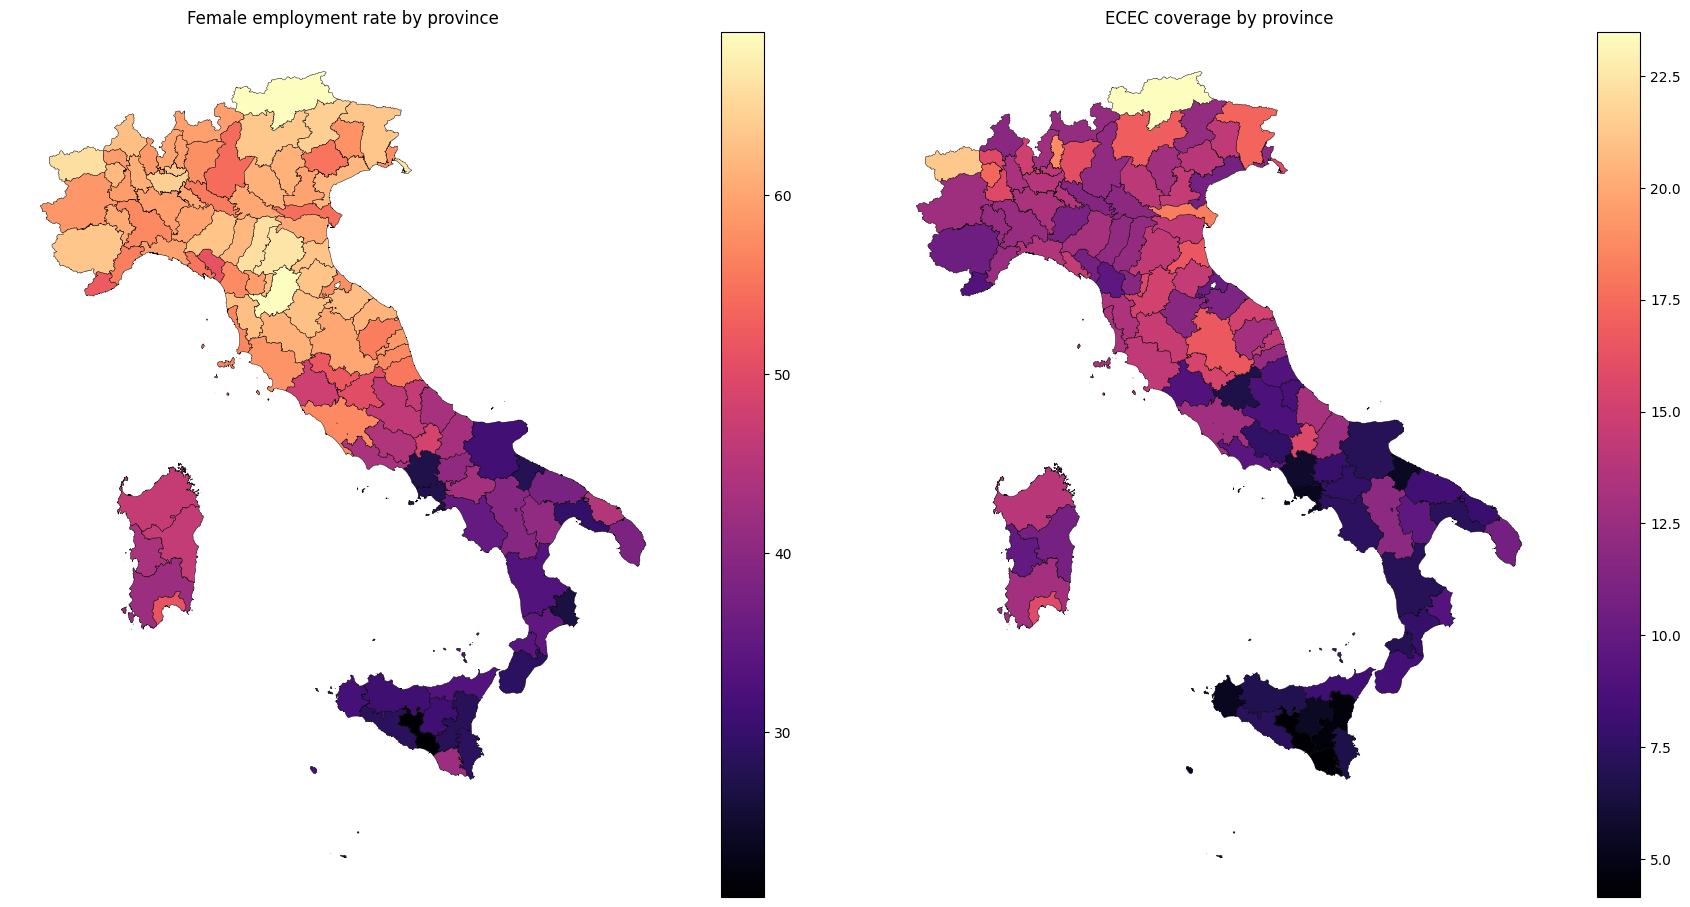
\includegraphics[width=0.9\linewidth]{chapters/images/fem_emp_rate_and_ECEC_map.png}
    \caption{Female employment rate (left) and ECEC coverage (right) by province heatmaps.}
    \label{fig:heatmap1}
\end{figure}

The heatmap clearly reveals two distinct regions, corresponding to Northern and Southern Italy. While the North exhibits peaks of women's employment reaching up to $69.1\%$, the South displays substantially lower values, with rates dropping to as low as $20.8\%$. Despite the relatively better performance of the North, Italy overall continues to record one of the lowest female employment rates in Europe.\\
The same holds for the coverage of ECEC services.\\

A positive association between women's employment and ECEC service indicators is suggested by visual inspection of the data and is formally confirmed by correlation analysis. We first compute a correlation matrix for the main employment and ECEC variables, and subsequently extend the analysis to all variables in the dataset. The results consistently indicate a strong positive correlation between women's employment rates and the provision and use of ECEC services. In particular, \texttt{fem\_empl\_rate} exhibits strong positive correlations with \texttt{per\_capita\_user\_contribution} (municipal expenditure per child financed by user contributions), \texttt{per\_capita\_public\_expenditure} (public expenditure per child), \texttt{coverage}, and \texttt{ecec\_participation} (percentage of children using ECEC services).\\

As exploratory measures of spatial autocorrelation, we compute Moran’s I (MI) \citep{Moran1950}, a global indicator ranging from $-1$ to $1$, where negative and positive values indicate negative and positive spatial autocorrelation, respectively. Statistical significance is assessed via a permutation test. For our variables of interest, we obtain $\text{MI} = 0.87$ for \texttt{fem\_empl\_rate} and $\text{MI} = 0.57$ for \texttt{coverage}, both indicating strong and statistically significant positive spatial autocorrelation.\\

To further investigate localized patterns of spatial dependence, we plot the Local Indicators of Spatial Association metric (LISA) using the local Moran's I \citep{Anselin1995} and generate cluster maps for the two variables, shown in Figure~\ref{fig:LISA}. The local Moran's I is a decomposition of the Global Moran's I statistic into individual values computed as: 

\begin{equation}   
    I_i = \frac{(Y_i - \bar Y)}{\sum_{j=1}^n (Y_i - \bar Y)^2/(n-1)}\sum^n_{j=1}w_{ij}(Y_j-\bar Y),
\end{equation}

where $Y_i$ is the value of a variable $Y$ in location \textit{i}, $\bar Y$ is the mean of $Y$, $n$ is the number of observations and $w_{ij}$ is the spatial weight between unit \textit{i} and \textit{j}. From the local Moran's I, we can check for the presence of clusters. Specifically, High--High (HH) and Low--Low (LL) clusters identify spatial concentrations of similarly high or low values (hotspots and coldspots, respectively), while High--Low (HL) and Low--High (LH) configurations indicate spatial outliers, where a province’s value contrasts with that of its surrounding area. This local analysis complements the global Moran’s I by highlighting heterogeneous spatial structures that are not captured by a single summary measure.\\

\begin{figure}[h] % THIS IMAGE LOOKS BLURED, WE NEED TO FIND A BETTER ONE
    \centering
    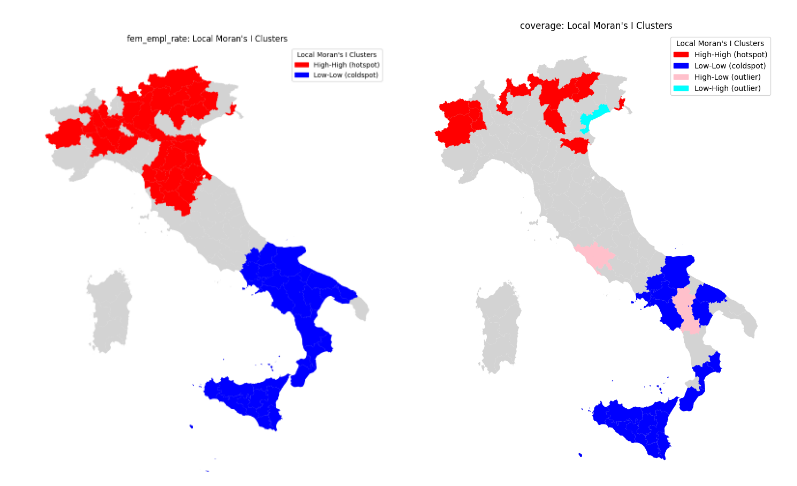
\includegraphics[width=0.9\linewidth]{Images/morans_clusters_inverted.png}
    \caption{LISA cluster map of \texttt{fem\_empl\_rate} (left) and \texttt{coverage} (right).}
    \label{fig:LISA}
\end{figure}


% Put a couple of comments about the EDA, expecially the part on correlation between covariates


\section{Preprocessing}
\label{sec:preprocessing}

Before fitting the models, we preprocess the data to make covariates comparable. Since predictors are measured on different scales, we standardize them using their sample means and standard deviations. In the rest of the analysis, we use the standardized predictors $X_{ij}^*$, for the j-th variable of the i-th province:

\begin{equation}
    X_{ij}^* = {{X_{ij} - \bar X_j} \over {s_{X_j}}}, \hspace{1cm} i = 1,..,N,  \hspace{0.5cm} j = 1,...,P
\end{equation}

Since the response $y_i = \texttt{fem\_empl\_rate}_i$ is a proportion, it takes values in $(0,1)$. To model it with a linear predictor, we apply a link function that maps $(0,1)$ to $\mathbb R$. In particular, we use the logit link, so we can model $y_i^*$ with a standard linear predictor:

\begin{equation}
    y_i^* = logit(y_i) = \log \bigg( {y_i \over {1 - y_i}} \bigg), \hspace{1cm} i = 1,...,N
\end{equation}

Unless otherwise stated, these preprocessing choices are adopted for the rest of the analysis.

\section{Variable Selection}
\label{sec:variable_selection}

Since the total number of numerical covariates is 47, we perform a variable selection procedure to identify the most relevant predictors $X_{ij}^*$ for the response $y_i^*$.\\

In a preliminary step, we drop specific variables deemed irrelevant by the sociological literature, most of which are related to the territorial characteristics of the provinces. Specifically, we drop: \texttt{urban\_type}, \texttt{area\_km2}, \texttt{internet\_coverage\_rate}, \texttt{green\_m2\_capita}, \texttt{eco\_urban\_index}.

Subsequently, we remove variables with a Pearson or Spearman's correlation coefficient $|\rho_{ij}| \ge 0.85$ with women's employment rate, such as \texttt{empl\_rate}, \texttt{unempl\_rate}, \texttt{inact\_rate}, \texttt{young\_neet}, \texttt{fem\_house\_rate}, \texttt{part\_rate}. Since the women's employment rate is the proportion of working women in working age, over all women of working age, all the aforementioned variables partially contain the same information, thus resulting in extremely high correlation coefficients.\\

Additionally, within each group of covariates (ECEC and non-ECEC), pairs of highly correlated variables are identified. For any pair with an absolute Pearson correlation coefficient $|\rho_{ij}| \ge 0.80$, one variable is discarded to mitigate multicollinearity. During this process, multiple variables are removed from the non-ECEC subset, such as \texttt{male\_edu\_rate}, dropped in favour of \texttt{fem\_edu\_rate}, \texttt{fertility\_rate} and \texttt{dependency\_rate}, which are dropped in favour of \texttt{ageing\_index}; finally, \texttt{GDP}, \texttt{foreign\_rate}, \texttt{adj\_net\_migration\_rate}, \texttt{n\_large\_comp}, and \texttt{house\_price} are removed, while \texttt{graduate\_mobility\_rate} is kept. Among the ECEC variables, we find that \texttt{other\_per\_capita\_expenditure} is virtually equal to \texttt{other\_percapita\_public\_expenditure}  ($|\rho_{ij}| = 0.99$). Additionally, \texttt{ecec\_participation} is highly correlated with both \texttt{per\_capita\_public\_expenditure} and \texttt{per\_capita\_user\_contribution}, which are highly correlated among themselves. Finally, \texttt{coverage} and \texttt{private\_coverage} show a high correlation, motivated by design, since $coverage_i = public\_coverage_i + private\_coverage_i$. For these reasons, we remove from our analysis the following ECEC variables: \texttt{coverage}, \texttt{per\_capita\_public\_expenditure}, \texttt{per\_capita\_user\_contribution} and \texttt{other\_per\_capita\_expenditure}.\\

After evaluating the variance inflation factor of the remaining variables, we note that most values are above 2, and some above 5\footnote{The table of VIF values can be inspected in Appendix A, table \ref{tab:vif_values}}.  We decide to apply a Bayesian Lasso approach \citep{Park2008} to perform further shrinkage and variable selection. The corresponding model specification, the distributions of $\beta_j$ coefficients (Figure \ref{fig:bayesian_lasso_results}) and the variables selected (Table \ref{tab:variable_selection_table}) are reported below:\\

\begin{align*}
    y^{\ast}_i \mid \boldsymbol{\beta}, \sigma, \phi_i 
        &\stackrel{\text{ind}}{\sim}\mathcal{N}\big(\alpha + \phi_i +  \boldsymbol{x}_i^{\ast \top} \boldsymbol{\beta},\, \sigma^2\big) \, ,
        \quad i = 1,\dots,N \\
    \beta_j \mid \lambda, \sigma 
        &\stackrel{\text{iid}}{\sim}\mathrm{Laplace}\big(0,\, \sigma / \lambda\big) \, ,
        \quad j = 1,\dots,P \\
    \lambda^2 &\sim \mathrm{Gamma}(2, 1), \\
    \sigma &\sim \mathrm{HalfNormal}(1), \\
    \alpha &\sim \mathcal{N}\big(0, \, 10^2),\\
    \phi \mid \tau_c, \rho, W &\sim \mathcal{N}_N \big(\boldsymbol{0},[\tau_c (D -\rho W)]^{-1} \big)\, \\
    \rho &\sim \mathrm{Beta}(2,2),\\
    \tau_c &\sim \mathrm{Gamma}(1,1).
\end{align*}\\

The Laplace prior can be expressed as a scale mixture of normals, leading to strong shrinkage of small coefficients toward zero while allowing relevant predictors to retain non-negligible effects. The global shrinkage parameter 
$\lambda$ controls the overall degree of penalization and is assigned a Gamma prior.\\

In addition, to account for residual spatial dependence in the response, we include a spatial random effect $\boldsymbol{\phi}$, modeled through a proper conditional autoregressive (CAR) prior. The structure matrix $(D - \rho W)$ is defined by the adjacency matrix $W$ of the areal units and the corresponding diagonal matrix $D$, where $D_{ii}$ equals the number of neighbors of province $i$. The parameter $\rho$ controls the strength of spatial autocorrelation, while $\tau_c$ governs the overall precision of the spatial effect. Weakly informative priors are adopted for $\alpha$ and $\sigma$, while $\rho$ and $\tau_c$ are assigned Beta and Gamma priors, respectively.\\

This formulation allows variable selection to be performed while simultaneously accounting for spatially structured unobserved heterogeneity, reducing the risk of selecting spurious covariates due to spatial autocorrelation in the residuals. The selection criteria adopted is to keep covariates that didn't include 0 in their 95\% CI.

\begin{table}[h]
    \centering
    \begin{tabular}{cc}
        \hline
        \textbf{ECEC variables} &  \textbf{Non-ECEC variables}\\
        \hline
        \texttt{private\_coverage} & \texttt{fem\_maj\_empl\_rate}\\
        \texttt{public\_coverage} & \texttt{service\_empl\_rate}\\
        \texttt{} & \texttt{graduate\_mobility\_rate}\\
        \texttt{} & \texttt{empl\_growth}\\
        
        \hline
    \end{tabular}
    \caption{Selected variables for the model.}
    \label{tab:variable_selection_table}
\end{table}

\begin{figure}[h]
    \centering
    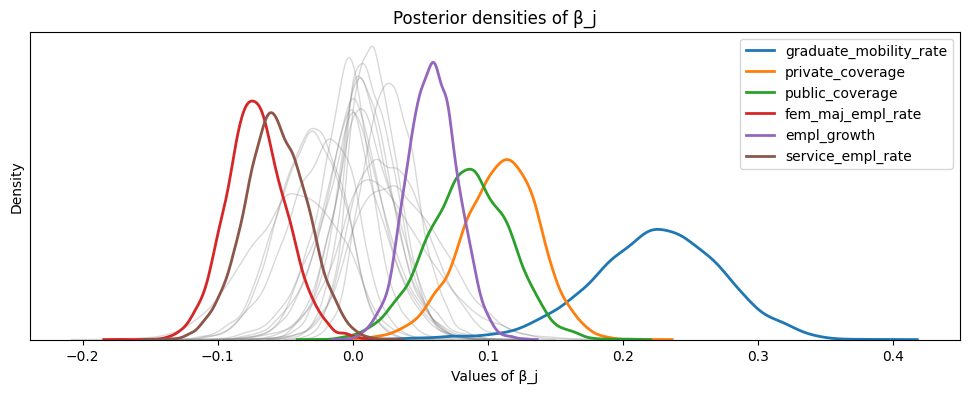
\includegraphics[width=0.9\linewidth]{chapters/images/final_variable_selection.png}
    \caption{Posterior densities of the coefficients $\beta_j$ and selected variables.}
    \label{fig:bayesian_lasso_results}
\end{figure}

\section{Model Specification}
\label{sec:models}
In this section, we introduce the Bayesian hierarchical model that allows for the study of spatial dependencies and uncovers the underlying clustering structure of areal data. The former is achieved by including spatial random effects via a CAR prior, while the latter is achieved by using finite mixtures with the number of components deliberately set high and a sparse prior on the weights favoring few non-empty components.

\subsection{Label Assignment}
\label{subsec:Label-Assignment}

The clustering model used in this study follows the idea of model-based clustering via sparse finite mixture models proposed by \cite{Malsiner-Walli2014}. Spatial heterogeneity is modeled by assuming that the regression coefficients take only a few distinct values across space. These distinct values define clusters of locations with similar covariate effects. The prior is designed to favor a small number of non-empty clusters, even when the upper bound on the number of mixture components is large.\\

We adopt a Gaussian likelihood for the logit-transformed employment rate $y^*$. Specifically, we consider a finite mixture model with $K$ components, where each component $k$ is characterized by its own regression coefficients $\beta_k$ and variance $\sigma_k^2$. A Dirichlet prior with concentration parameter smaller than one is assigned to the vector of mixture weights $\pi$, encouraging sparsity in the mixture distribution. As a result, the posterior typically allocates mass to only a subset of the $K$ components. Finally, a spatial random effect $\phi_i$ is included to account for residual spatial autocorrelation through a CAR-Leroux prior\footnote{CAR prior distribution implementation in Stan is presented in Appendix B.}. The mean-centering constraint is employed since it helps avoid an identifiability issue (confounding) with the intercept \citep{duncan2024developing}.\\

Let $i=1,\dots,N$ index observations, $j=1,\dots,P$ covariates, and $k=1,\dots,K$ mixture components. Let $\mathbf{x}_i^\ast \in \mathbb{R}^P$ be the $i$-th row of $X^\ast$, and $y_i^\ast$ the logit transformed response. Define the known graph matrix $W\in[0,1]^{N\times N}$ and degree matrix $D=\mathrm{diag}(d_1,\dots,d_N)$ with $d_i=\sum_{i'=1}^N W_{ii'}$.

\begin{align*}
y_i^\ast \mid \alpha,\boldsymbol{\pi},\{\boldsymbol{\beta}_k,\sigma_k^2\}_{k=1}^K,\phi_i
&\stackrel{\text{ind}}{\sim} \sum_{k=1}^K \pi_k\,
\mathcal{N}\!\Big(\alpha+\mathbf{x}_i^{\ast\top}\boldsymbol{\beta}_k+\phi_i,\ \sigma_k^2\Big),
\qquad i=1,\dots,N\\[2mm]
\boldsymbol{\pi} &\sim \mathrm{Dirichlet}\!\big(0.5\,\mathbf{1}_K\big),\\
\alpha &\sim \mathcal{N}(0,2),\\
\beta_{j,k}\mid b_{j,k},\lambda_{j}
&\stackrel{\text{ind}}{\sim} \mathcal{N}\!\Big(b_{j,k},\ \lambda_{j} \Big),
\qquad j=1,\dots,P,\ k=1,\dots,K\\
b_{j} &\stackrel{\text{iid}}{\sim} \mathcal{N}(0,1),
\qquad j=1,\dots,P\\
\lambda_{j} &\stackrel{\text{iid}}{\sim} \mathrm{Gamma}(0.5,0.5), \,
\qquad j=1,\dots,P\\
\sigma^2_k = \frac{1}{\nu_k}, \qquad \nu_k &\stackrel{\text{iid}}{\sim} \mathrm{Gamma}(2,1),
\qquad k=1,\dots,K\\
\phi_i &= \phi_{\mathrm{raw},i}-\frac1N\sum_{i'=1}^N \phi_{\mathrm{raw},i'},
\qquad i=1,\dots,N\\
\boldsymbol{\phi}_{\mathrm{raw}}\mid \tau,\rho,W
&\sim \mathcal{N}_N\!\Big(
\mathbf{0},\ \big[\tau\{\rho(D-W)+(1-\rho)I_N\}\big]^{-1}
\Big),\\
\tau &\sim \mathrm{Gamma}(2,1),\\
\rho &\sim \mathrm{Beta}(1,1).
\end{align*}

\subsubsection{Posterior Cluster Allocation in \texttt{Stan}}
Let $z_i \in \{1,\dots,K\}$ denote the latent label of province $i$. For each province $i$ and component $k$, we compute the component-specific mean:
\[
\mu_{ik} \;=\; \alpha + \mathbf{x}_i^{*\top}\boldsymbol{\beta}_k + \phi_i, \qquad i=1,\dots,N,\ k=1,\dots,K
\]
We then compute the unnormalized allocation weights:
\[
w_{ik} \;=\; \pi_k\, \mathcal{N}\!\big(y_i^* \mid \mu_{ik}, \sigma_k^2\big), 
\qquad i=1,\dots,N,\ k=1,\dots,K
\]
and normalize them to obtain probabilities:
\[
r_{ik} \;=\; \frac{w_{ik}}{\sum_{h=1}^K w_{ih}},
\qquad i=1,\dots,N,\ k=1, \dots,K
\]
Finally, we sample the label as:
\[
z_i \mid \mathbf{r}_i \;\sim\; \mathrm{Categorical}(\mathbf{r}_i),
\qquad i=1,\dots,N
\]
where $\mathbf{r}_i=(r_{i1},\dots,r_{iK})$.
This produces one complete label vector $\mathbf{z}=(z_1,\dots,z_N)$ for each posterior draw.

\subsubsection{Posterior Similarity Matrix}
Directly averaging the labels over iterations is not meaningful, since component labels can switch across draws.
A standard label-invariant summary is the posterior similarity matrix (PSM), defined by:
\[
S_{ii'} \;=\; \Pr(z_i=z_{i'} \mid \text{data}), \qquad 1\le i<i'\le N
\]
Let $\mathbf{z}^{(1)},\dots,\mathbf{z}^{(M)}$ be the $M$ label draws obtained from the procedure above.
We estimate the PSM by:
\[
\widehat{S}_{ii'}
\;=\;
\frac{1}{M}\sum_{m=1}^M \mathbb{I}\!\left(z_i^{(m)} = z_{i'}^{(m)}\right), \qquad 1\le i<i'\le N
\]
Large values of $\widehat{S}_{ii'}$ indicate that provinces $i$ and $i'$ are frequently assigned to the same cluster in the posterior.

\subsubsection{Point Estimate of the Partition via Binder Loss}

For interpretation we need a single representative partition.
We obtain it by minimizing the posterior expected Binder loss \cite{Binder_1978}.
Given a candidate label vector $\hat{\mathbf{z}}$, the Binder loss is
\[
L_{\mathrm{Binder}}(\mathbf{z},\hat{\mathbf{z}})
\;=\;
\sum_{i<i'}
\Big(
a\,\mathbb{I}(z_i=z_{i'})\,\mathbb{I}(\hat{z}_i\neq \hat{z}_{i'})
\;+\;
b\,\mathbb{I}(z_i\neq z_{i'})\,\mathbb{I}(\hat{z}_i=\hat{z}_{i'})
\Big),
\]
where $a>0$ is the cost of incorrectly separating a pair and $b>0$ is the cost of incorrectly merging a pair.
The posterior expectation of $L_{\mathrm{Binder}}$ depends on the PSM.
Using $S_{ii'}=\Pr(z_i=z_{i'}\mid\text{data})$, we have
\[
\mathbb{E}\!\left[L_{\mathrm{Binder}}(\mathbf{z},\hat{\mathbf{z}})\mid \text{data}\right]
=
\sum_{i<i'}
\Big(
a\,S_{ii'}\,\mathbb{I}(\hat{z}_i\neq \hat{z}_{i'})
+
b\,(1-S_{ii'})\,\mathbb{I}(\hat{z}_i=\hat{z}_{i'})
\Big).
\]
Minimizing the posterior expected Binder loss defines the optimal partition $\hat{\mathbf{z}}$. The resulting partition defines the final cluster labels used in the next subsection.

\subsection{Full Hierarchical Model}
\label{subsec:full_model}
Let $C$ be the number of non-empty clusters in the chosen partition $\hat{\mathbf z}$ and denote by $c_i \in \{1,\dots,C\}$ the assigned cluster for province $i$.
Conditional on $\mathbf c=(c_1,\dots,c_N)$, the mixture representation is no longer needed and the
model becomes a standard hierarchical regression with cluster-specific parameters.
In particular, each cluster $c$ is associated with a coefficient vector $\boldsymbol{\beta}_c$
and a residual scale $\sigma_c$.



\begin{align*}
y_i^\ast \mid \alpha,\boldsymbol{\beta}_{c_i},\phi_i,\sigma_{c_i}
&\stackrel{\text{ind}}{\sim} \mathcal{N}\!\Big(\alpha+\mathbf{x}_i^{\ast\top}\boldsymbol{\beta}_{c_i}+\phi_i,\ \sigma_{c_i}^{2}\Big),
\qquad i=1,\dots,N\\[2mm]
\alpha &\sim \mathcal{N}(0,2),\\
\beta_{j,c}\mid b_{j,c},\lambda_{j}
&\stackrel{\text{ind}}{\sim} \mathcal{N}\!\Big(b_{j,c},\ \lambda_{j} \Big),
\qquad j=1,\dots,P,\ c=1,\dots,C\\
b_{j,c} &\stackrel{\text{iid}}{\sim} \mathcal{N}(0,1),
\qquad j=1,\dots,P,\ c = 1,\dots,C\\
\lambda_{j} &\stackrel{\text{iid}}{\sim} \mathrm{Gamma}(0.5,0.5), \,
\qquad j=1,\dots,P\\
\sigma^2_c = \frac{1}{\nu_c}, \qquad \nu_c &\stackrel{\text{iid}}{\sim} \mathrm{Gamma}(2,1),
\qquad c=1,\dots,C\\
\phi_i &= \phi_{\mathrm{raw},i}-\frac1N\sum_{i'=1}^N \phi_{\mathrm{raw},i'} \, ,
\qquad i=1,\dots,N\\
\boldsymbol{\phi}_{\mathrm{raw}}\mid \tau,\rho,W
&\sim \mathcal{N}_N\!\Big(
\mathbf{0},\ \big[\tau\{\rho(D-W)+(1-\rho)I_N\}\big]^{-1}
\Big),\\
\tau &\sim \mathrm{Gamma}(2,1),\\
\rho &\sim \mathrm{Beta}(1,1).
\end{align*}
\section{Results and Discussion}
In this section we report the results obtained from the label-assignment step described in Section \ref{subsec:Label-Assignment} and the final model fit described in Section \ref{subsec:full_model}, using the covariates selected in
Chapter \ref{sec:variable_selection}. Moreover, Appendix C presents a validation study on synthetic data, illustrating the model’s performance.

\subsection{Posterior Cluster Allocation}
\label{subsec:clusters}

Following Section \ref{subsec:Label-Assignment}, we generated posterior draws of the latent allocation labels and summarized the clustering structure in a label-invariant way through the posterior similarity matrix (PSM) and a point estimate of the partition obtained via Binder loss.\\

The posterior evidence indicates that the model assigns all provinces to a single cluster. Equivalently, the estimated partition has $C=1$ non-empty component, so that no spatially distinct groups with different regression effects are detected. In practical terms, this means that the data do not support heterogeneous covariate effects across provinces under the proposed mixture/CAR specification and prior settings.\\

Given $C=1$, the full hierarchical model in Section \ref{subsec:full_model} reduces to a standard spatial regression with a single global coefficient vector $\beta$ (and residual scale $\sigma$), while spatial dependence is captured by the CAR random effect $\phi$:
\begin{align}
y_i^* \mid \alpha,\beta,\phi_i,\sigma &\sim \mathcal{N}\!\left(\alpha + x_i^{*\top}\beta + \phi_i,\ \sigma^2\right),
\qquad i=1,\dots,N.
\end{align}
All posterior summaries reported in the following sections refer to this $C=1$ fit.

\subsection{Posterior Inference}

\subsubsection{Predictors}

Table~\ref{tab:post_betas} reports posterior summaries for the intercept and regression coefficients associated with the covariates selected in Chapter \ref{sec:variable_selection}.

\begin{table}[!ht]
\centering
\begin{tabular}{lrrrrr}
\toprule
Parameter & Mean & SD & 5\% & 50\% & 95\% \\
\midrule
Intercept ($\alpha$) & 0.053 & 0.021 & 0.020 & 0.053 & 0.087 \\
private\_coverage & 0.104 & 0.037 & 0.044 & 0.105 & 0.165 \\
fem\_maj\_empl\_rate & -0.080 & 0.031 & -0.130 & -0.081 & -0.029 \\
public\_coverage & 0.151 & 0.034 & 0.095 & 0.150 & 0.206 \\
service\_empl\_rate & -0.059 & 0.031 & -0.110 & -0.059 & -0.008 \\
graduate\_mobility\_rate & 0.254 & 0.046 & 0.177 & 0.255 & 0.327 \\
empl\_growth & 0.051 & 0.027 & 0.007 & 0.051 & 0.094 \\
\bottomrule
\end{tabular}
\caption{Posterior summaries for intercept and regression coefficients.}
\label{tab:post_betas}
\end{table}

Figure~\ref{fig:dens_betas} shows posterior density estimates for the regression coefficients. This visualization complements Table~\ref{tab:post_betas}.\\

\begin{figure}[!ht]
\centering
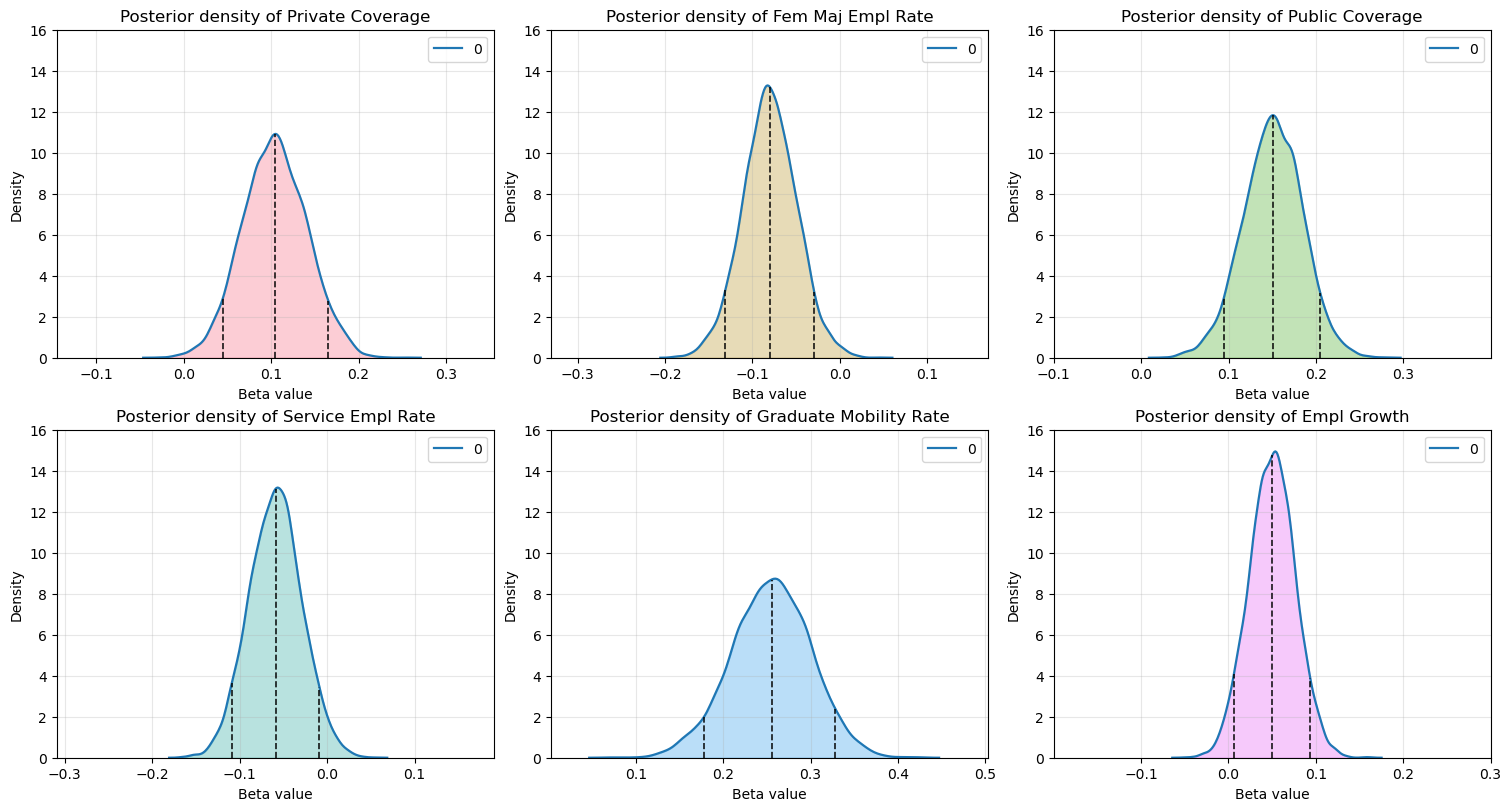
\includegraphics[width=\textwidth]{chapters/images/posterior-density-plots.png}
\caption{Posterior densities for the intercept and regression coefficients.}
\label{fig:dens_betas}
\end{figure}


According to Table~\ref{tab:post_betas} and Figure~\ref{fig:dens_betas}, the covariate showing the strongest positive association is the \texttt{graduate\_mobility\_rate}. This result is plausible, as female employment rates tend to be higher in provinces containing large urban areas with abundant job opportunities, which are also characterized by higher graduate mobility.\\

In addition, both private and public coverage variables are likewise positively correlated with the female employment rate. This finding was expected and it's encouraging for our study, although it does not allow us to establish a causal relationship between coverage and the increase in female employment.\\

In contrast, \texttt{fem\_maj\_empl\_rate} and \texttt{service\_empl\_rate} appear to be negatively correlated with female employment. However, compared with the other predictors, these effects are less significant.\\


\subsubsection{Spatial effect}

The response exhibits strong spatial autocorrelation. To interpret CAR random effect $\boldsymbol\phi$, we compare its posterior mean with the observed response.
Figure~\ref{fig:phi_vs_y} reports the posterior mean map of $\mathbb{E}[\phi_i\mid y]$, and the province-level \texttt{fem\_empl\_rate}. Provinces with positive (negative) $\phi_i$ correspond
to areas where the employment rate is systematically higher (lower) than what is explained by the selected covariates alone, after accounting for overall intercept and noise. In other words, $\boldsymbol\phi$ captures residual spatial patterns not explained by the included predictors.

\begin{figure}[!ht]
\centering
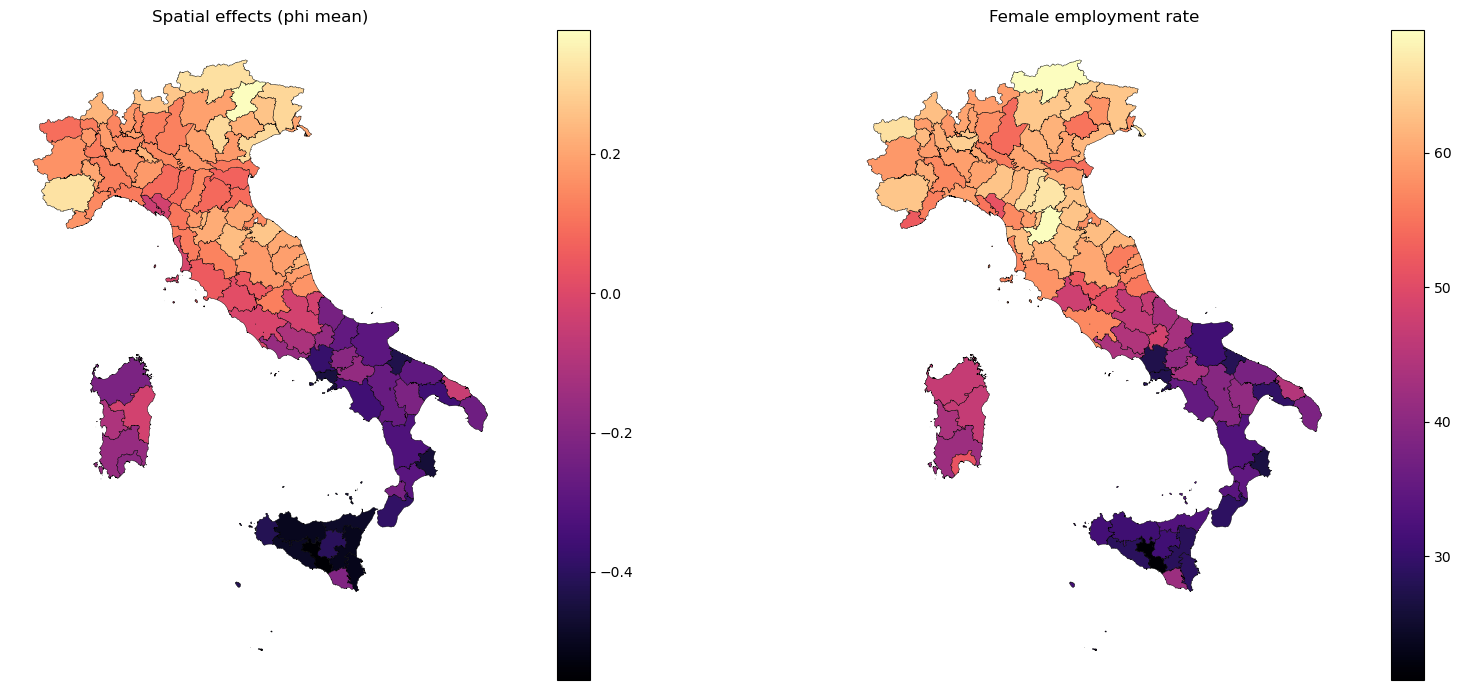
\includegraphics[width=0.85\textwidth]{chapters/images/car-vs-fem.png}
\caption{Posterior mean of the spatial random effects $\boldsymbol\phi$ (left) and Observed female employment rate by province (right).}
\label{fig:phi_vs_y}
\end{figure}

From Figure~\ref{fig:phi_vs_y}, we observe that the spatial effect across Italy follows the same overall trend as the female employment rate, with a gradual divide between the northern and southern provinces. This suggests the presence of a significant underlying structure that is not explained by the selected predictors. 
\section{Conclusions and Future Work}
\label{sec:conclusions}

This work studied provincial differences in female employment in Italy (year 2022) and their relationship with ECEC availability and socio-economic covariates, using a Bayesian spatial modeling framework with a CAR random effect and a sparse finite mixture approach for model-based clustering.\\

The label-assignment step resulted in a single cluster including all provinces, indicating no posterior support for distinct groups characterized by different regression effects. Consequently, inference is effectively that of a global spatial regression: associations between the selected covariates and female employment are summarized through one coefficient vector, while remaining geographic disparities are
captured by the spatial random effect.\\

Future work could extend the analysis in several directions, one option could be repeating the study over multiple years to increase statistical power to detect heterogeneous relationships and enable joint spatio-temporal modeling. Another option would be to enrich the dataset with additional covariates (not correlated with the others we already have) that capture further drivers of the outcome, thereby improving explanatory power and reducing the share of variation absorbed by the spatial effect.\\


% REMEMBER TO REMOVE NOCITE{*} FROM THE BIB, OTHERWISE THERE ARE PAPERS WE DIDN'T USE IN THE BIB

% DO NOT CSAY THAT WE SELECTED THE MODEL BECAUSE OF THE BINDER LOSS

\newpage
\bibliography{bibliography.bib}

\newpage
\section*{Appendix A: List of Variables}
\label{sec:appendix_a}

Table~\ref{tb:variables_list} presents the complete list of variables in the dataset and their description:

\begin{table}[H]
    \small
    \centering
    \makebox[\textwidth][c]{
    \begin{tabularx}{1.1\textwidth}{ >{\hsize=0.7\hsize}X >{\hsize=1.3\hsize}X}
    \hline
    \textbf{Variable} & \textbf{Description}\\
    \hline
    fem\_empl\_rate & Employed women (15-64) / Total women (15-64)\\
    population & Residents on January $1^{st}$\\
    unempl\_rate & Unemployed (15-64) / Labor force (15-64)\\
    \textbf{part\_rate} & Labor force (15-89) / Population (15-89)\\
    empl\_rate & Employed (15-64) / Labor force (15-64)\\
    \textbf{empl\_growth} & Annual growth of employed population\\
    inact\_rate & Inactive (15-64) / Population (15-64)\\
    \textbf{fem\_edu\_rate} & Women 20+ with tertiary education\\
    \textbf{male\_edu\_rate} & Men 20+ with tertiary education\\
    \textbf{service\_empl\_rate} & Workers in service (15-64) / All workers\\
    \textbf{GDP} & Gross Domestic Product at market prices per person\\
    \textbf{n\_large\_comp} & Local units with 250+ employees / Active population (in thousands)\\
    \textbf{n\_self\_empl} & Number of self-employed / Active population\\
    young\_neet & 15-29 not in employement, education or training / 15-29 people\\
    \textbf{fem\_house\_rate} & Inactive women / Children aged 0-2\\
    \textbf{foreign\_rate} & Foreigners / Total population\\
    n\_members\_family & Average numer of members per family\\
    elderly\_in\_care & 65+ in home or interated care services\\
    house\_price & Average price per housing (€/$m^2$)\\
    fertility\_rate & Live births per 1000 residents\\
    first\_birth\_maternal\_age & Average age at first childbirth\\
    avg\_children\_per\_woman & Total fertility rate (TFR)\\
    dependency\_rate & Non-working / Working-age population\\
    ageing\_index & 65+ / 0-14 population\\
    net\_migration\_rate & Net migration per 1000 residents\\
    adj\_net\_migration\_rate & Migration adjusted for natural change\\
    area\_km2 & Total surface area\\
    public\_transport\_supply & Public transport supply per capita\\
    internet\_coverage\_rate & \% on households with high-speed internet\\
    graduate\_mobility\_rate & Net migration of graduates (25-39)\\
    green\_m2\_capita & Green space per capita in provincial capitals\\
    eco\_urban\_index & Environmental performance score\\
    \textbf{per\_capita\_public\_expenditure} & Municipal spending per 0-2 years old\\
    ecec\_participation & \% of 0-2 years old using early childhood services\\
    \textbf{coverage} & Number of available children services / Children aged 0-2\\
    urban\_type & 1: Urban, 2: Intermediate, 3: Rural\\
    \textbf{per\_capita\_user\_contribution} & Per-child user spending (€ per 0-2 years old)\\
    \textbf{advanced\_business\_empl} & Employees in advanced business services per active population\\
    lifelong\_learn & \% of population aged 25-64 in lifelong learning\\
    startup\_ratio & Innovative startups per 1000 corporations\\
    \textbf{fem\_maj\_empl\_rate} & Workers in Education and Health and Social Care / All workers\\
    \hline
    \end{tabularx}
    }
    \caption{List of numerical variables present in the data. Highlighted rows show computed variables, not directly taken.}
    \label{tb:variables_list}
\end{table}

\newpage
Figure \ref{fig:scatterplot} reports a pairwise scatterplot matrix for the outcome ($\texttt{fem\_empl\_rate}$) and ECEC variables. The diagonal panels show the marginal distributions of each variable, while the lower panels display the corresponding bivariate relationships and the higher ones displays correlation values. Observations are colored by Italian macro-area ($\texttt{rip\_name}$), highlighting geographic heterogeneity and potential North–South differences in both covariate distributions and associations with female employment:

\begin{figure}[h]
    \centering
    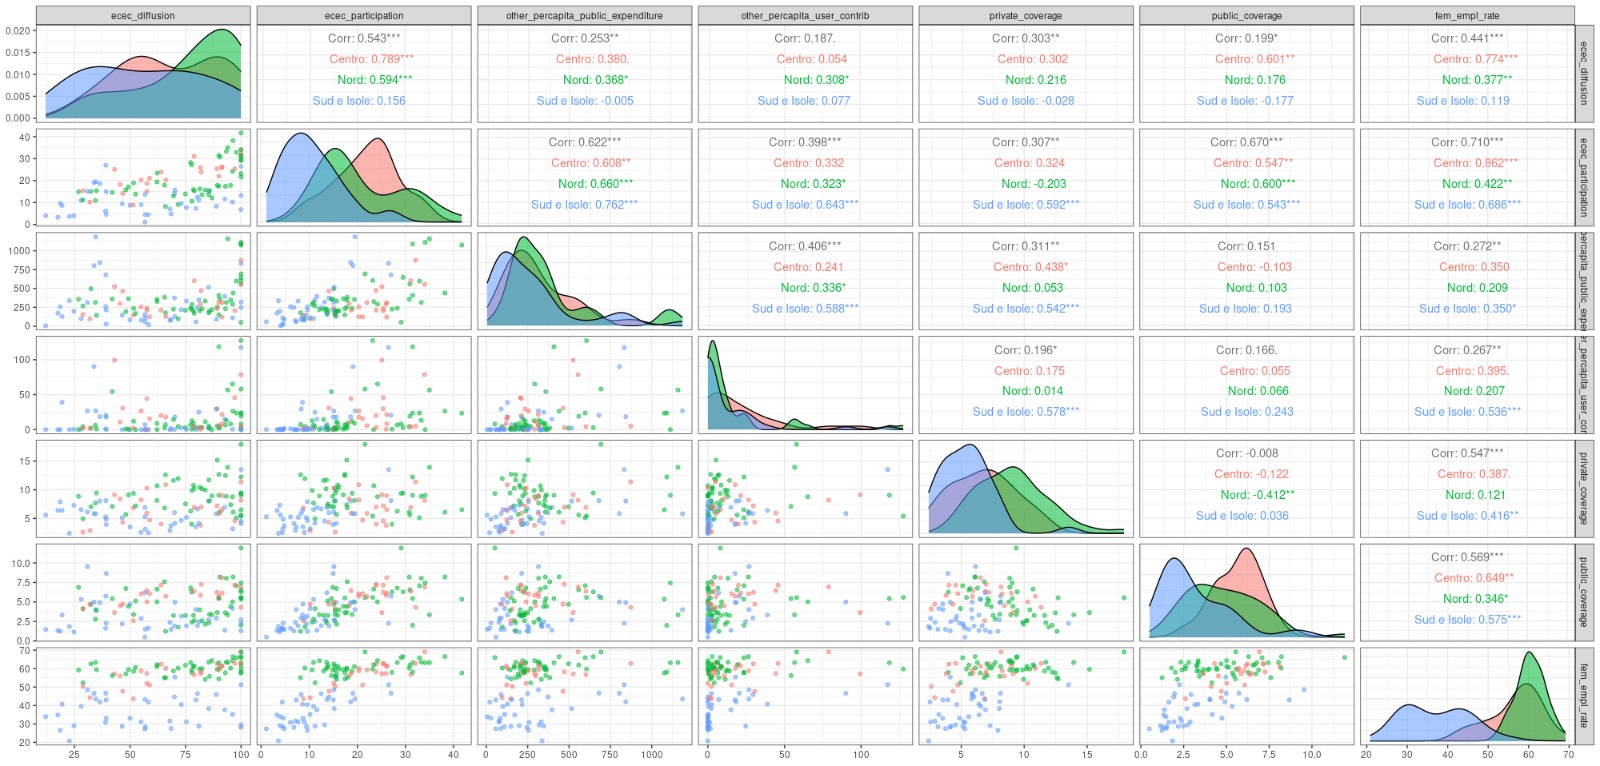
\includegraphics[width=\linewidth]{chapters/images/scatterplots.jpeg}
    \centering
    \caption{Pairwise scatterplot matrix of the main variables used in the study.\\
    \texttt{rip\_name}: Blue = South and Islands, Green = North, Red Center.\\}.
    \label{fig:scatterplot}
\end{figure}

Table~\ref{tab:vif_values} reports the VIF values of the potential covariates before performing Bayesian LASSO.

\begin{table}[h]
\centering
\caption{VIF values of potential covariates before Bayesian LASSO.}
\label{tab:vif_values}
\begin{tabular}{lc}
\hline
\textbf{variable} & \textbf{VIF} \\
\hline
ecec\_participation & 9.140282 \\
graduate\_mobility\_rate & 8.102231 \\
advanced\_business\_empl & 7.346519 \\
n\_members\_family & 6.564543 \\
ageing\_index & 6.548976 \\
public\_coverage & 4.139228 \\
first\_birth\_maternal\_age & 4.010305 \\
fem\_edu\_rate & 3.987515 \\
other\_percapita\_public\_expenditure & 3.876044 \\
avg\_children\_per\_woman & 3.464354 \\
public\_transport\_supply & 3.437207 \\
population & 3.238429 \\
GERD\_total\_intramural & 3.057367 \\
ecec\_diffusion & 2.517609 \\
lifelong\_learn & 2.359288 \\
service\_empl\_rate & 2.229131 \\
private\_coverage & 2.186444 \\
n\_self\_empl & 1.833873 \\
startup\_ratio & 1.784709 \\
other\_percapita\_user\_contrib & 1.684447 \\
fem\_maj\_empl\_rate & 1.503210 \\
elderly\_in\_care & 1.347364 \\
empl\_growth & 1.319513 \\
\hline
\end{tabular}
\end{table}

\newpage
\section*{Appendix B: CAR Leroux prior in Stan}\label{ann:lpdf_car}

Since the proper CAR Leroux prior is not directly available in \texttt{Stan}, we implement it by explicitly defining its log probability density function (lpdf). In this appendix, we derive the expression of the lpdf corresponding to the CAR Leroux prior, defined as:
\[
\boldsymbol{\phi}_{\mathrm{raw}} \mid \tau,\rho,W
\sim \mathcal{N}_N\!\Big(
\mathbf{0},\ 
\big[\tau\{\rho(D-W)+(1-\rho)I_N\}\big]^{-1}
\Big),
\]
where $W$ denotes the adjacency matrix, $D$ is the diagonal matrix of neighborhood counts,\\
i.e. $D_{ii}=\sum_j W_{ij}$, $\tau$ is the precision parameter, and $\rho\in[0,1]$ controls the degree of spatial dependence.\\

Define the matrices $V=\rho(D-W)+(1-\rho)I_N$ and $Q=\tau V$.
Then, the CAR Leroux prior can be written as:
\[
\boldsymbol{\phi} \mid \tau,\rho,W
\sim \mathcal{N}_N\!\left(\mathbf{0},\, Q^{-1}\right).
\]
The corresponding density is:
\[
\pi(\boldsymbol{\phi} \mid W,\tau,\rho)
= (2\pi)^{-N/2}\det(Q)^{1/2}
\exp\!\left(-\tfrac12 \boldsymbol{\phi}^\top Q \boldsymbol{\phi}\right).
\]
Ignoring constants that do not depend on the parameters, the log-density is proportional to:
\begin{align}
\log \pi(\boldsymbol{\phi} \mid W,\tau,\rho)
&\propto \tfrac12 \log \det(Q)
- \tfrac12 \boldsymbol{\phi}^\top Q \boldsymbol{\phi} \nonumber\\
&= \tfrac12 \log \det(\tau V)
- \tfrac{\tau}{2}\boldsymbol{\phi}^\top V \boldsymbol{\phi} \nonumber\\
&= \tfrac{N}{2}\log(\tau)
+ \tfrac12 \log \det(V)
- \tfrac{\tau}{2}\boldsymbol{\phi}^\top V \boldsymbol{\phi}.
\label{eq:log_density_car}
\end{align}

We now derive an expression for $\det(V)$.
Since $D-W$ is symmetric, it admits the eigendecomposition:
\[
D-W = U \Lambda U^\top,
\]
where $U$ is orthogonal and $\Lambda=\mathrm{diag}(\lambda_1,\dots,\lambda_N)$.
Therefore:
\[
V=\rho(D-W)+(1-\rho)I_N
=U\big(\rho\Lambda+(1-\rho)I_N\big)U^\top.
\]
Hence, the eigenvalues of $V$ are $\rho\lambda_i+(1-\rho)$, $i=1,\dots,N$, and we define the following result for $det(V)$:
\begin{equation}
\det(V)
= \prod_{i=1}^N \big(\rho\lambda_i + 1-\rho\big).
\label{eq:detV}
\end{equation}

Substituting Eq.\eqref{eq:detV} into Eq.\eqref{eq:log_density_car}, we obtain
\begin{align}
\log \pi(\boldsymbol{\phi} \mid W,\tau,\rho)
&\propto
\tfrac{N}{2}\log(\tau)
+ \tfrac12 \sum_{i=1}^N \log\big(\rho\lambda_i + 1-\rho\big)
- \tfrac{\tau}{2}\boldsymbol{\phi}^\top V \boldsymbol{\phi}.
\label{eq:log_density_final}
\end{align}

Equation Eq.\eqref{eq:log_density_final} is implemented in \texttt{Stan} to define the custom lpdf for the CAR Leroux prior.

\newpage
\section*{Appendix C: Simulation study}\label{subsec:sim-study}

We present a simulation study to assess the ability of the proposed model to correctly estimate the parameters and the clustering of the areal units. Using the model introduced in Section \ref{subsec:Label-Assignment}, we simulate data for a grid of $10 \times 10$ areal units.

The adjacency structure is induced by contiguity on the grid (units are treated as neighbors if they share a boundary). The spatial effect $\phi_i$ is simulated fixing $\tau = 1$ and $\rho = 0.9$. Conditional on a fixed true partition, each unit $i$ is assigned a vector of covariates $x_i \in \mathbb{R}^{P}$, with $P=2$ in the implementation, generated independently from a Gaussian distribution. Given the true cluster membership $k \in \{1,\dots,K_0\}$, the response is then generated from a cluster-specific linear regression model:
\[
y_i = \phi_i + x_i^\top \beta_{k} + \varepsilon_i \, , 
\qquad \varepsilon_i \sim \mathcal{N}(0,1),
\]
where $\beta_k$ varies across clusters. In the experiments below we report results for two configurations of the true cluster structure (a simpler setting with $K_0=4$ clusters and a more complex setting with $K_0=7$ clusters), corresponding to the maps displayed in Figures~\ref{fig:true-vs-pred-k4} and \ref{fig:true-vs-pred-k7}.

Posterior sampling is carried out via Hamiltonian Monte Carlo using four chains, 5,000 warm-up iterations and 5,000 retained iterations per chain. Cluster labels are produced at each posterior draw through the label-assignment step described in Section~\ref{subsec:Label-Assignment}.\\

Figure~\ref{fig:psm} shows a clear block-diagonal structure in the PSM, indicating that the posterior assigns high co-clustering probability to units within the same true region, while keeping between-region probabilities close to zero. This qualitative pattern is reflected in the spatial maps: in the simpler $K_0=4$ setting, the estimated partition aligns perfectly with the ground truth (Figure~\ref{fig:true-vs-pred-k4}). Moreover the density plots (Figure \ref{fig:betaposterior-true}) show that the true $\beta$ coefficients are accurately recovered.

In the more heterogeneous configuration, the selected partition yields $K=7$ clusters and recovers the overall structure (Figure~\ref{fig:true-vs-pred-k7}). Discrepancies are limited to a small subset of units and are concentrated at the borders between neighboring clusters; in addition, the distinction between two true clusters is essentially lost, as these regions are largely merged into a single estimated cluster in the predicted map.


\begin{figure}[H]
  \centering
  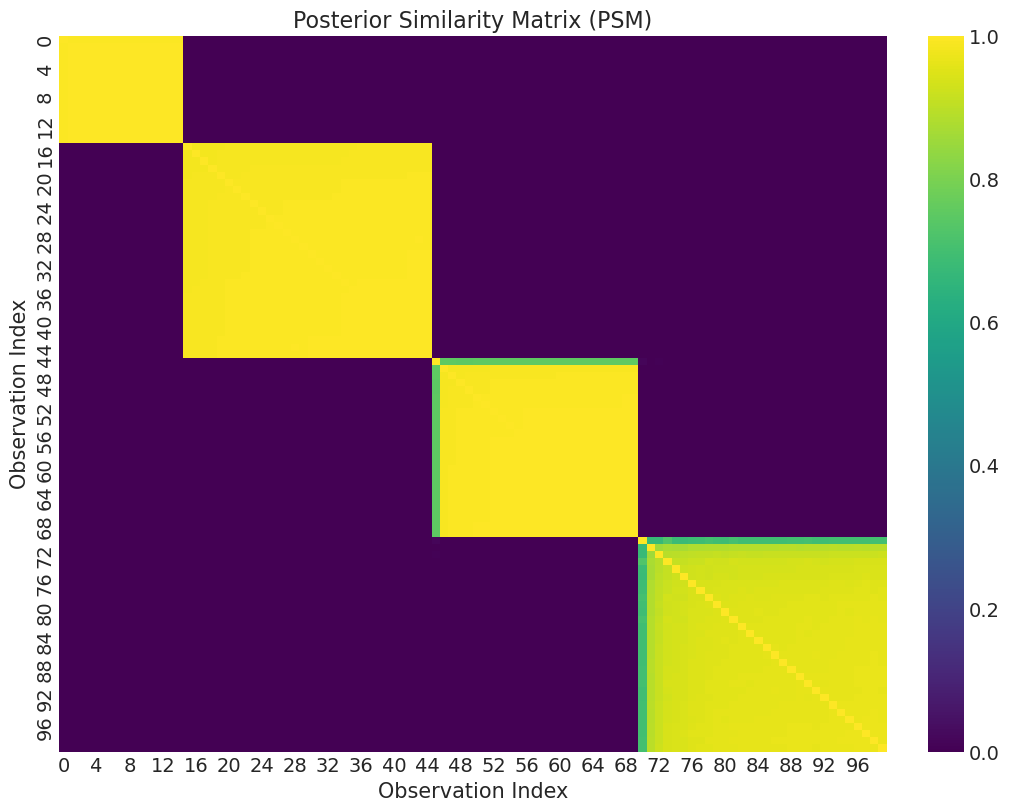
\includegraphics[width=0.65\textwidth]{chapters/images/psm-k4.png}
  \caption{Posterior similarity matrix (PSM) for the simulated data when $K_0 = 4$.}
  \label{fig:psm}
\end{figure}

\begin{figure}[H]
  \centering
  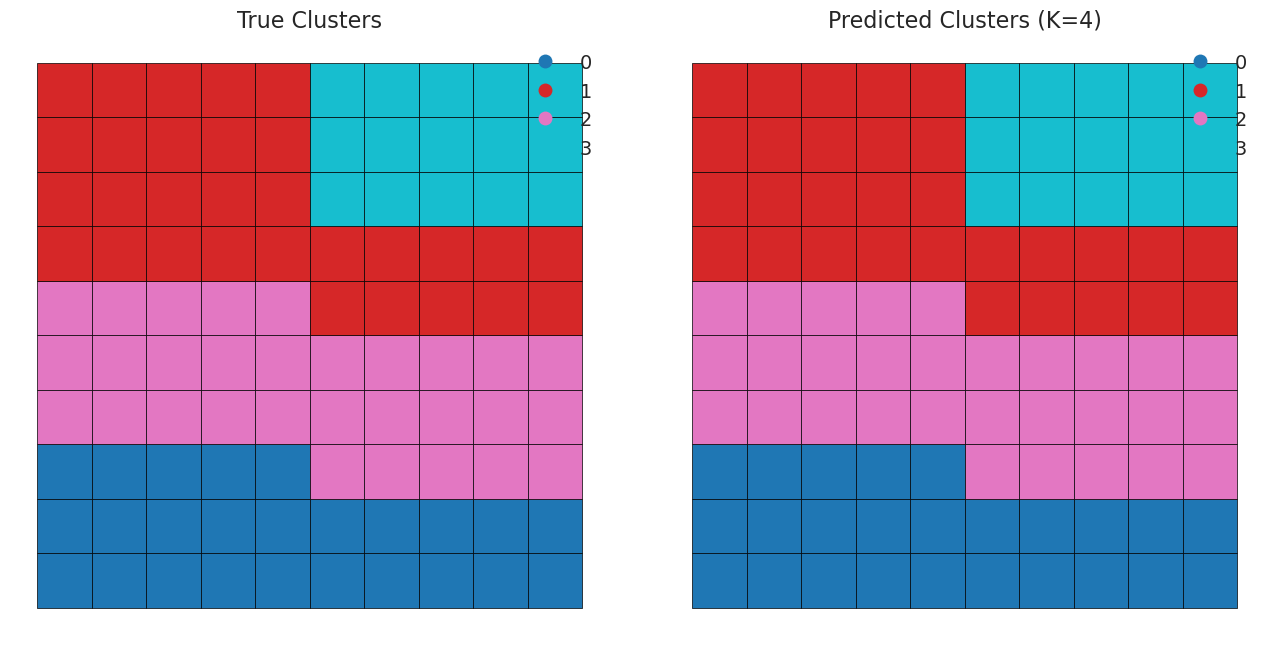
\includegraphics[width=0.8\textwidth]{chapters/images/comparison-k4.png}
  \caption{True clusters (left) and estimated clusters (right) for the $K_0=4$ configuration.}
  \label{fig:true-vs-pred-k4}
\end{figure}

\begin{figure}[H]
  \centering
  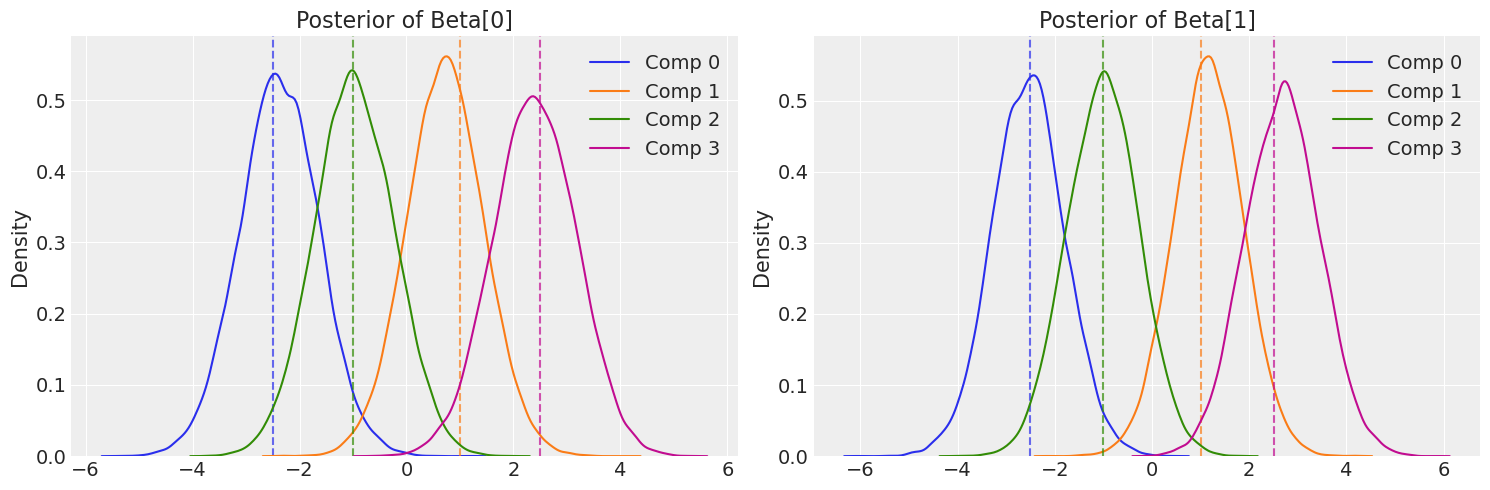
\includegraphics[width=1\textwidth]{chapters/images/betaposterior-truevalue.png}
  \caption{Posterior density of the cluster-specific regression coefficients $\beta$ and their true value for the $K_0 = 4$ configuration.}
  \label{fig:betaposterior-true}
\end{figure}

\begin{figure}[htbp]
\centering
  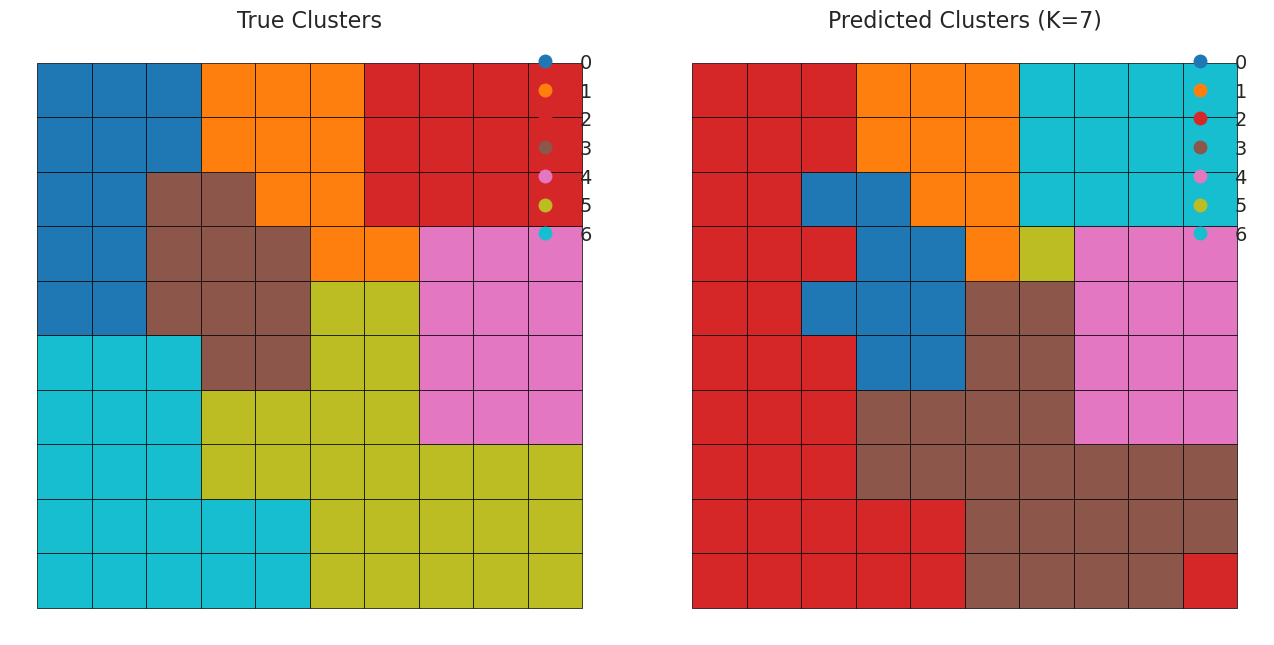
\includegraphics[width=0.8\textwidth]{chapters/images/comparison-k7.png}
  \caption{True clusters (left) and estimated clusters (right) for the for the configuration with $K_0 = 7$.}
  \label{fig:true-vs-pred-k7}
\end{figure}





\end{document}